\section{Motor Friction Estimation}
\label{sec:motor_friction_estimation}

This section details the estimation of the motor friction coefficients using a pendulum model. The pendulum is used to measure the motor friction coefficients by measuring the angular velocity and acceleration of the pendulum as it is released from a known initial angle. The friction coefficients are then estimated using linear regression.




\subsection{Pendulum Modeling}

The pendulum used in the motor friction tests consists of an aluminum rod of length \( l_{\text{arm}} = 0.19 \) meters and a ballast mass \( m_{\text{ballast}} = 0.301 \) kg attached at a distance \( r = 0.08 \) meters from the pivot. The total mass of the arm is \( m_{\text{arm}} = 0.034 \) kg. The pendulum is modeled as a rigid body rotating about the motor shaft with a moment of inertia \( I \) given by:

\[
I = \frac{1}{3} m_{\text{arm}} l_{\text{arm}}^2 + m_{\text{ballast}} r^2
\]

The equation of motion for the pendulum, considering only viscous friction, is:

\[
I \ddot{\theta} + b \dot{\theta} + (m_{\text{arm}} \frac{l_{\text{arm}}}{2} + m_{\text{ballast}} r) g \sin(\theta) = 0
\]

where:
\begin{itemize}
    \item \( \theta \) is the angular displacement (positive counterclockwise, zero at vertical down position)
    \item \( \dot{\theta} \) and \( \ddot{\theta} \) are the angular velocity and acceleration, respectively
    \item \( b \) is the viscous damping coefficient
    \item \( g = 9.81 \, \text{m/s}^2 \) is the acceleration due to gravity
\end{itemize}

\subsection{Linear Regression Derivation}
Rearranging the equation for linear regression purposes:

\[
    I \ddot{\theta} + (m_{\text{arm}} \frac{l_{\text{arm}}}{2} + m_{\text{ballast}} r) g \sin(\theta) = -b \dot{\theta}
\]

This can be expressed in the form:

\[
Y = X \beta
\]

where:
\begin{itemize}
    \item \( Y = -I \ddot{\theta} - (m_{\text{arm}} \frac{l_{\text{arm}}}{2} + m_{\text{ballast}} r) g \sin(\theta) \),
    \item \( X = \dot{\theta} \),
    \item \( \beta = b \).
\end{itemize}

The angular velocity \( \dot{\theta} \) and acceleration \( \ddot{\theta} \) are computed using centered finite differences:

\[
\dot{\theta}_i = \frac{\theta_{i+1} - \theta_{i-1}}{2\Delta t}
\]

\[
\ddot{\theta}_i = \frac{\theta_{i+1} - 2\theta_i + \theta_{i-1}}{(\Delta t)^2}
\]

where \(\Delta t\) is the time step between measurements.

The linear least squares solution for \( \beta \) is given by:

\[
\beta = (X^T X)^{-1} X^T Y
\]

This yields the viscous damping coefficient \( b \).

The viscous damping coefficient \( b \) is found to be \( 0.001 \) Nm/rad/s for the hip motors (A20 etc) and \( 0.0001 \) Nm/rad/s for the knee motors (A14 etc).

A plot of the data and the linear regression fit is shown in figure \ref{fig:results:motor_friction_estimation:linear_regression}.

\begin{figure}[h]
    \centering
    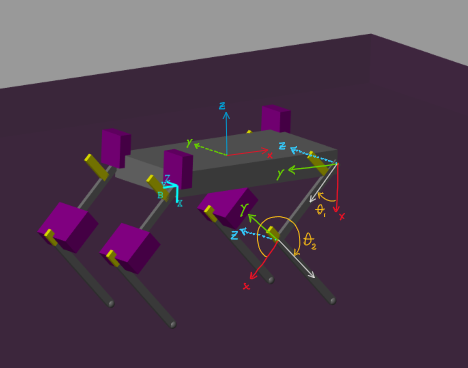
\includegraphics[width=0.8\textwidth]{Images/angle_conventions.png}
    \caption{Linear regression fit of the pendulum data.}
    \label{fig:results:motor_friction_estimation:linear_regression}
\end{figure}

TODO: Switch figure \ref{fig:results:motor_friction_estimation:linear_regression} to the correct figure, I just want to compile for now. 